%% \chapter[htoc-titlei][hhead-titlei]{htitlei}
%% -----------------------------------------------------------------------------
\chapter[Prospects for same-sign $WW$ at the High Luminosity LHC][Prospects for same-sign $WW$ at the High Luminosity LHC]{Prospects for same-sign $WW$ at the High Luminosity LHC}
\label{ch:sswwupgrade}

%Over the course of the next eight years, the LHC and ATLAS will go through two scheduled extended maintenance periods--the Phase-I and Phase-II upgrades--in which the experiment will be upgraded to the High Luminosity LHC (HL-LHC)

On December 3, 2018, Run 2 of the LHC officialy ended, and the collider was shut down to begin the first of two scheduled extended maintenance periods \cite{2018.cern-press-run2}.
During these two long shutdowns, the Phase-I and Phase-II upgrades of the LHC and ATLAS will occur in order to prepare for the High-Luminosity LHC (HL-LHC) which is scheduled to begin operation in 2026 \cite{2011.atlas-phase1-loi}.

The HL-LHC is planned to run at a center-of-mass energy of \com{14} with an instantaneous luminosity of $\mathcal{L}=5\times 10^{34}~\textrm{cm}^{-2}\textrm{s}^{-1}$ with up to 200 collisions per beam-crossing. 
Over the course of operation, the HL-LHC is expected to collect a total integrated luminosity of $\mathcal{L} = 3000~\mathrm{fb}^{-1}$ by 2035 \cite{2015.hllhc-design-report}.

These run conditions are much harsher than what ATLAS has experienced so far, and as a result there are several planned upgrades to the detector.
Most notably, the entire ID will be replaced with an all-silicon tracker which will extend the coverage from $|\eta| \le 2.7$ up to $|\eta| \le 4.0$.
This will allow for reconstruction of charged particle tracks which can in turn be matched to clusters in the calorimeters for electron identification or forward jet tagging \cite{2015.atlas-phase2-scoping}.
%There are also plans for additional muon detectors at high rapidity

%While the HL-LHC is still years in the future, it is 
The upgraded detector combined with the higher beam energy and the considerable increase in integrated luminosity means that many analyses with low signal statistics in Run 2 have the potential to be greatly improved with the HL-LHC.
While the ATLAS 13~TeV \ssww cross section measurement certainly did not suffer greatly from low statistics \TODO{--reword--}, the accuracy of the measurement can still be improved at the HL-LHC. % would it become ``systematics limited'' instead of ``statistics limited'' -- look into this, could be good to say if so.
%Additionally, there are expected to be enough signal events to measure the polarization of the produced $W$ bosons.
Of particular interest is the longitudinal polarization of the $W$ bosons due to its sensitivity to electroweak symmetry breaking~\cite{2013.longitudinal-theory}.% which is expected to be measurable for the first time.

The analysis detailed in this chapter is based off of the 2018 public ATLAS \ssww prospects study~\cite{2018.ssww-upgrade} which is itself an extension of the 2017 ATLAS study~\cite{2017.ssww-upgrade}.  \TODO{mention CMS's study + yellow report?}


% overview of the analysis
\subsection{Analysis Overview}
% define signal in workds
The experimental signature of interest is identical to the $13\tev$ analysis: two prompt leptons (either electrons or muons) with the same charge, missing transverse energy, and two high energy, forward jets.
These jets are again required to have a large angular separation and a high combined invariant mass to preferentially select EWK- over QCD-produced \ssww events.

% introduce key backgrounds
Background processes are again similar to the $13\tev$ analysis and are summarized again here. %i am assuming prompt and non-prompt will be defined in the 13 TeV section
The dominant source of prompt background from $WZ$+jets events where both bosons decay leptonically.  
If the lepton from the $Z$-decay with opposite charge from the $W$ falls outside of the detector acceptance or is not identified, the remainder could appear to be a \ssww signal event.
To a lesser extent, $ZZ$+jets events can enter the signal region in much the same way provided two leptons are ``lost''.
Other prompt sources include $t\bar{t}+V$ and and multiple parton interactions, however these processes do not contribute much.
These prompt backgrounds are expected to contribute less than in Run 2 with the addition of forward tracking in the upgraded ATLAS detector.
Jets mis-reconstructed as leptons or leptons from hacronic decays (such as $t\bar{t}$ and $W$+jets production) comprise the non-prompt lepton background.
Lastly, events with two prompt, opposite-charge electrons can appear as a same-sign event provided one of the electrons is mis-reconstructed as the wrong charge.

% goals of analysis -- xsec, polarization, optimization
In this analysis, the EWK production of \ssww is studied in the context of the planned HL-LHC run conditions and upgraded ATLAS detector.
An optimized event selection (referred to as the \emph{optimized selection}) is also explored in an effort to gain increased signal significance over the \emph{default selection}.
The cross section of the inclusive EWK production is measured for both the default and optimized selections, and the extraction of the longitudinal scattering significance is measured with the optimized selection.


% I don't think we need enough detail on the hllhc upgrades to warrant its own section, we can just mention the main impacts (forward tracking, luminosity, etc)
%\section{HL-LHC Upgrades}\label{sswwupgrade:hllhc}
%\input{sections/ssww_upgrade/hllhc.tex}

\section{Theoretical motivation}\label{sswwupgrade:theory}
The theoretical motivation for studying the ssWW process is detailed in Section~\ref{ssww13tev:vbs_theory}.
\TODO{Re-write this section referencing the main description in the 13tev section. Maybe just turn this into a 1 or 2 sentence refresher}
The particular interest in polarization is the potential for the scattering amplitude of longitudinally polarized weak bosons to diverge linearly as the center of mass energy increases, ultimately violating unitarity around $1\tev$ \cite{1977.ben-lee-weak-interactions}.
In the Standard Model, the Higgs boson cancels these divergences.
However, as the Higgs is recently discovered it is still extremely to study the mechanism of electroweak symmetry breaking (EWSB), and the longitudinal scattering of $W$ bosons is expected to be one of the most sensitive tests of EWSB~\cite{2013.longitudinal-theory}.

%some additional detail on the interest in the longitudinally polarized $W$ bosons follows \cite{2016.ssww-polarization, 2013.longitudinal-theory, 2017.multiboson-at-lhc}.

\subsection{Experimental sensitivity to longitudinal polarization}\label{sec:sswwupgrade_longitudinal_sens}
\TODO{mention that since there are so many polarization possibilities, a large integrated luminosity is needed to measure just one of them individually}
There are three possible polarization states for a massive vector boson: two transverse ($+$ or $-$) and one longitudinal ($0$).
Therefore, in a system with two $W$ bosons, the overall polarization can be purely longitudinal ($00$), purely transverse ($++$, $--$, and $+-$), or mixed ($+0$ and $-0$).
The three combinations will be referred to as \emph{LL}, \emph{TT}, and \emph{LT} respectively.

In order extract the longitudinal scattering component, it is necessary to find variables that distinguish the LL from the TT and LT.
Several variables were studied, and those with the best discriminating power between the polarizations were the leading and subleading lepton $\pt$ as well as the azimuthal separation ($|\dphijj|$) of the two VBS jets.
The LL events preferred lower $\pt$ for both signal leptons (see Figure~\ref{fig:polarization_leppt}), which motivates keeping these two cuts as low as possible in the event selection in order to preserve as much longitudinal polarization as possible.
In the case of $|\dphijj|$, the LL events generally had a larger dijet separation (see Figure~\ref{fig:polarization_dphijj}), and this variable is used in a binned likelihood fit to extract the longitudinal scattering significance.

\begin{figure}[htp]
  \centering
  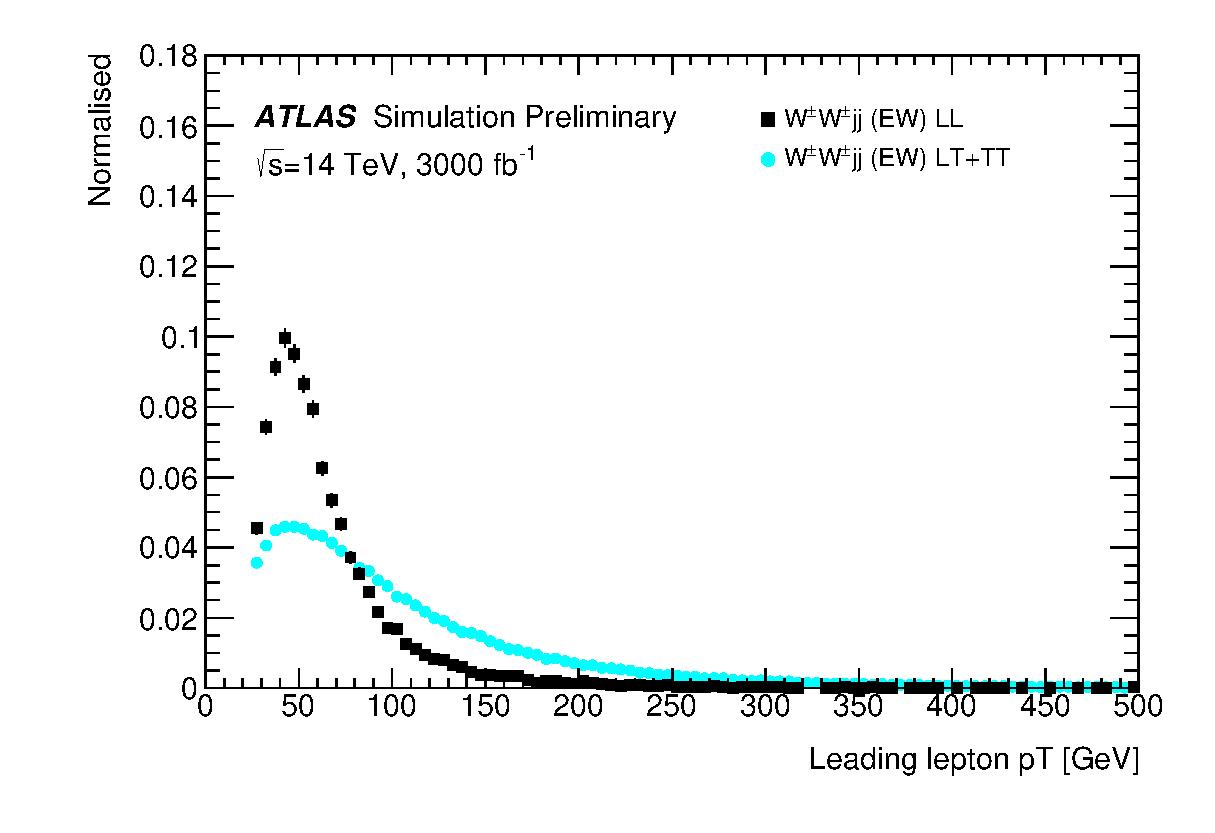
\includegraphics[width=0.8\textwidth]{figs/ssww_upgrade/polarization/lepton0_pt_pass9}\\
  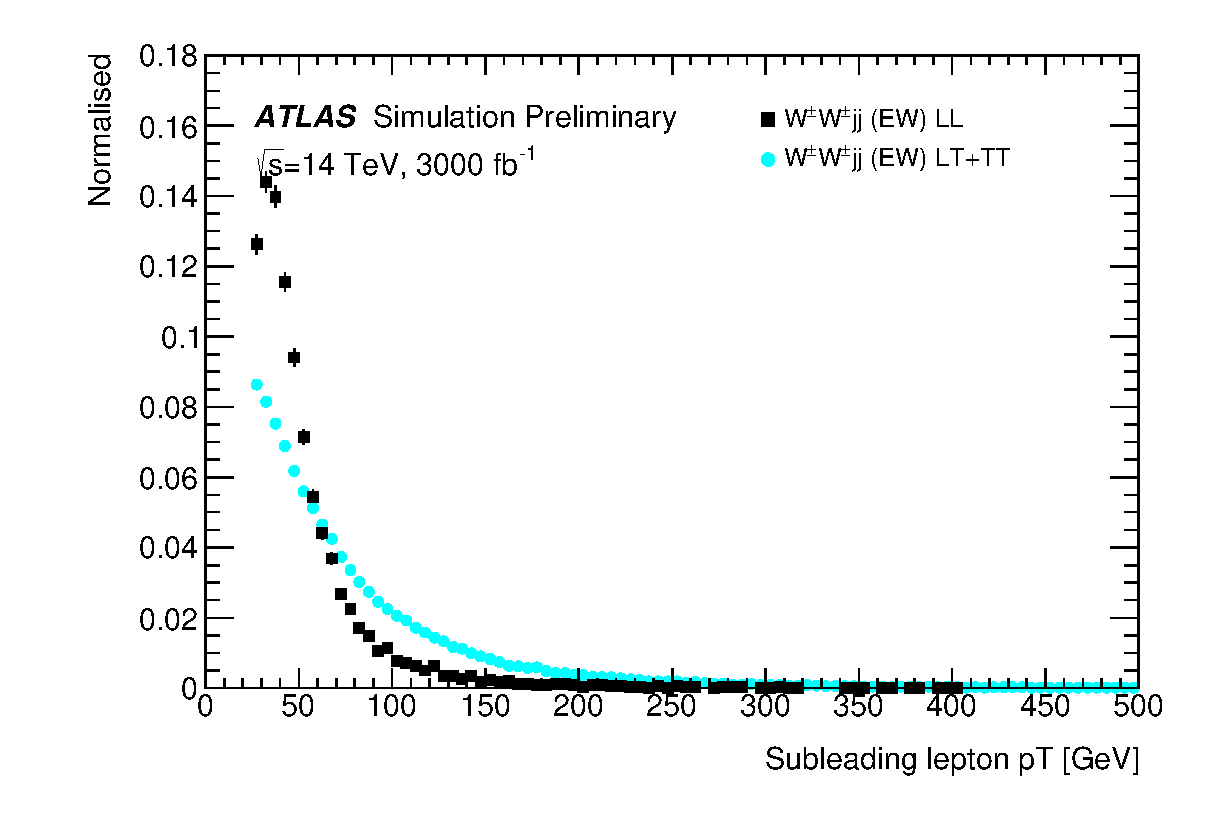
\includegraphics[width=0.8\textwidth]{figs/ssww_upgrade/polarization/lepton1_pt_pass9}
  \caption{Comparison of the leading (top) and subleading (bottom) lepton $\pt$ distributions for purely longitudinal (LL, black) and mixed polarization (LT+TT, cyan) \ssww events.}
  \label{fig:polarization_leppt}
\end{figure}

\begin{figure}[htp]
  \centering
  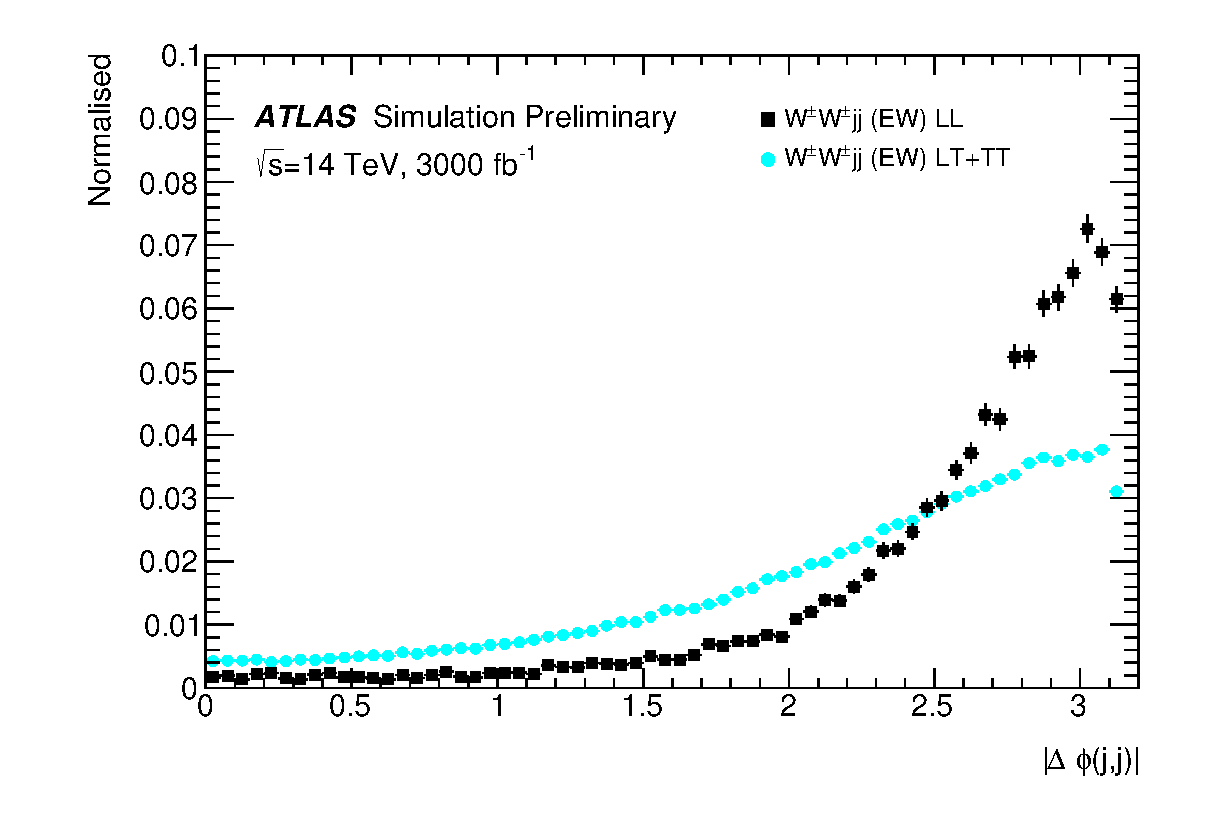
\includegraphics[width=0.8\textwidth]{figs/ssww_upgrade/polarization/dijet_absdphijj_pass9}
  \caption{Comparison of the azimuthal dijet separation ($|\dphijj|$) for purely longitudinal (LL, black) and mixed polarization (LT+TT, cyan) \ssww events.}
  \label{fig:polarization_dphijj}
\end{figure}

% gains from increase in cross sections of signal/background -- this could just be put in the section introduction/hllhc upgrades
% polarization theory only?

\section{Monte Carlo samples}\label{sswwupgrade:mc}
As no real HL-LHC data will be available for many years, all processes in this prospects study must be simulated using Monte Carlo (MC) generators. 
Signal and background processes were generated at \com{14}, and the event yields scaled to the anticipated HL-LHC integrated luminosity of $\mathcal{L}=3000~\textrm{fb}^{-1}$.

\TODO{Consider putting all this in a table}

%signal
The signal sample consists of both VBS and non-VBS electroweak (EWK) \ssww production, and it is sumulated with the \mcatnlo generator \cite{2014.madgraph_mcnlo} using the \nnpdf PDF set \cite{2015.NNPDF3} and interfaced with \pythiav{8} \cite{2015.pythia82} for hadronization and parton showering.
To study the longitudinal polarization more directly, two additional \mcatnlo \ssww samples are used: one containing only the longitudinal contribution (LL) and a second containing the transverse (TT) and mixed (LT) contributions.

%background
\TODO{Here we talk about things that mimic the experimental signature before we formally state what the signal is...}
There are many other processes that can produce the same final state as the \ssww and must also be accounted for using MC simulations.
$WZ$ events are generated using \sherpav{2.2.0} \cite{2009.Sherpa, 2008.CS_Shower, 2009.METS}, which includes up to one parton at next-to-leading order (NLO) in the strong coupling constant $\alpha_s$ and up to three additional partons at leading order (LO).  
Both EWK and QCD production are included in these samples.
$ZZ$ events are generated using \sherpav{2.2.2} with up to two additional partons in the final state.
Triboson backgrounds $VVV, V = W, Z$ where the bosons can decay leptonically or hadronically are simulated with \sherpav{2.2.2} with up to two additional partons in the final state.
$W$+jets backgrounds are generated for electron, muon, and tau final states are generated at LO with \mcatnlo and the \nnpdf set with showering from \pythiav{8}.
$Z$+jets events are generated using \powhegbox \cite{2010.powhegbox} and the \ctten PDF set \cite{2010.ct10} interfaced with \pythiav{8}.
Finally, $t\bar{t}$ and single-top events are generated using \powhegbox with showering from \pythiav{6}.

Since the MC samples used in the analysis are generated at particle-level and have not been run through the typical full simulation of the ATLAS detector, smearing functions are instead used to estimate detector effects.
These are derived from a \tt{GEANT4} simulation of the detector \cite{2003.GEANT4}.
%All MC samples are generated at particle-level, and detector effects are estimated using smearing functions derived from a full simulation of the ATLAS detector in \tt{GEANT4} \cite{2003.GEANT4}.
%Pileup events are fully simulated.


%\section{Signal definition}\label{sswwupgrade:signal}
%Hello world!

\subsection{Sensitivity to longitudinal polarization}


\section{Background estimations}\label{sswwupgrade:background}
\TODO{MC samples, what we estimate directly from MC, Charge flip, fakes, and isolation}

\subsection{Truth based isolation}\label{sec:sswwupgrade_isolation}


\section{Object and event selection}\label{sswwupgrade:object_event_selection}
\TODO{Add table for full lepton (pre-)selection, full jet (pre-)selection, and then finally the overall event selection}

\begin{table}[htb]
  \centering
  \begin{tabular}{l|c}
    Selection requirement              & Selection value \\
    \hline\hline
    \multirow{2}{*}{Lepton kinematics} & $\pt > 25$~GeV \\
                                       & $|\eta| \le 4.0$ \\
    \multirow{2}{*}{Jet kinematics}    & $\pt > 30$~GeV for $|\eta| \le 4.5$ \\
                                       & $\pt > 70$~GeV for $|\eta| > 3.8$ \\
    \hline
    Dilepton charge                    & Exactly two signal leptons with same charge\\
    Dilepton separation                & $\Delta R_{l,l} \ge 0.3$ \\
    Dilepton mass                      & $m_{ll} > 20$~GeV\\
    $Z$ boson veto                     & $|m_{ee} - m_Z| > 10$~GeV ($ee$-channel only) \\
    $\met$                             & $\met > 40$~GeV \\
    Jet selection                      & At least two jets with $\Delta R_{l,j} > 0.3$\\
    $b$ jet veto                       & $N_{\textrm{b-jet}} = 0$\\
    Dijet separation                   & $\detajj > 2.5$\\
    Trilepton veto                     & No additional preselected leptons\\
    Dijet mass                         & $m_{jj} > 500$~GeV\\
    Lepton-jet centrality\footnote{$\zeta = \min [\min (\eta_{\ell1}, \eta_{\ell2} )-\min(\eta_{j1},\eta_{j2}), \max(\eta_{j1},\eta_{j2})-\max(\eta_{\ell1},\eta_{\ell2}) ]$}                                    & $\zeta > 0$\\
    \hline
  \end{tabular}
  \caption{derp}
  \label{tab:sswwupgrade_event_selection}
\end{table}


\section{Selection optimization}\label{sswwupgrade:optimization}
%The \ssww upgrade study is a good opportunity to try to optimize the signal event selection.
As mentioned earlier, the HL-LHC will feature forward tracking, an increase in center of mass energy, and a higher integrated luminosity.
Therefore, this study is an excellent time to see if there are new optimizations to the signal event selection that can improve the signal to background ratio.

%------------------------------------------------------------------------------------------------------
%
%------------------------------------------------------------------------------------------------------
\subsection{Random grid search algorithm}\label{sswwupgrade:opt_rgs}
The chosen method for optimizing the event selection is a cut-based algorithm known as the Random Grid Search (RGS) \cite{2018.rgs-paper}.
Consider a simple case of two variables $x$ and $y$ chosen to differentiate the signal from the background.
In order to be considered a signal event, a given event would be required to pass a \emph{cut point} $c = \{x > x_c, y > y_c\}$.
A simple method to choose the optimal cut point (i.e. the ``best'' values of the cuts $x_c$ and $y_c$) would be to construct an $n\times m$ rectangular grid in $x$ and $y$ consisting of points $(x_0,y_0), (x_1,y_1), ..., (x_n,y_m)$, as in Figure~\ref{fig:rgs_square_grid}.
One can then choose a cut point $c_k = \{x > x_i, y > y_j\}$ that maximizes the signal significance as measured by a chosen metric.
This would be considered a \emph{regular} or \emph{rectangular} grid search.

While effective in principle, this rectangular grid search comes with two major drawbacks:
\begin{enumerate}
\item The algorithm does not scale well as the number of variables to be optimized--the dimensionality of the grid--increases.  In the case of a square grid with $N$ bins per variable $v$, the number of cut points to be evaluated grows as $N^v$.
\item Signal and background samples are rarely evenly distributed over the entire grid, resulting in many cut points being sub-optimal and evaluating them would be a waste of computing resources.
\end{enumerate}

To combat these limitations, the RGS algorithm constructs a grid of cut points directly from the signal sample itself.
In the two-dimensional example, this means that the variables $x_i$ and $y_j$ making up the cut point $c_k = \{x > x_i, y > y_j\}$ take their values directly from a given signal event.
This has the benefit of creating a \emph{random grid} of cut points that is by construction  biased towards regions of high signal concentration.
This reduces the need for exponentially increasing numbers of cut points while ensuring that computing resources are not wasted in regions with few to no signal events.
An example of the the two-dimensional random grid is shown in Figure~\ref{fig:rgs_random_grid}.

\begin{figure}[htp]
  \centering
  \includegraphics[width=0.48\textwidth]{figs/ssww_upgrade/rgs/figures_cuts_regulargrid}
  \caption{A visual representation of a rectangular grid search algorithm.  The signal events are the blue triangles, and the red circles are the background events. \TODO{replace with own figure}}   
  \label{fig:rgs_square_grid}
\end{figure}

\begin{figure}[htp]
  \centering
  \includegraphics[width=0.48\textwidth]{figs/ssww_upgrade/rgs/figures_cuts_randomgrid}
  \caption{A visual representation of a random grid search algorithm.  The signal events are the blue triangles, and the red circles are the background events.  \TODO{replace with own figure}}   
  \label{fig:rgs_random_grid}
\end{figure}

Once the random grid of cut points is constructed, the optimal cut point can be chosen using whatever metric the analyzer chooses, such as signal to background ratio.
For the purpose of the \ssww upgrade study, the optimal cut point is the one that mazimizes the signal significance $Z$ defined as in Equation~\ref{eq:significance_with_error} \cite{2011.asimov-significance}.
\begin{equation}
Z = \sqrt{2{\bigg[}(s+b)\ln{\Big(}\frac{s+b}{b_0}{\Big)}+b_0-s-b{\bigg]}+\frac{(b-b_0)^2}{\sigma_b^2}}
\label{eq:significance_with_error}
\end{equation}
where $s$ and $b$ are the number of signal and background events, respectively, $\sigma_b$ is the total uncertainty on the background, and $b_0$ is defined as:
\begin{equation}
b_0 = \frac{1}{2}{\Big(}b-\sigma_b^2+\sqrt{(b-\sigma_b^2)^2+4(s+b)\sigma_b^2}{\Big)}
\label{eq:significance_b0}
\end{equation}

In the case where the backround is known precisely (i.e. $\sigma_b = 0$), Equation~\ref{eq:significance_with_error} simplifies to
\begin{equation}
Z = \sqrt{2\bigg(b\big[(1+s/b)\ln(1+s/b)-s/b\big]\bigg)}
\label{eq:significance_without_error}
\end{equation}
which further reduces to the familiar $Z = s/\sqrt{b}$ for the case when $s << b$.

%------------------------------------------------------------------------------------------------------
%
%------------------------------------------------------------------------------------------------------
\subsection{Inputs to the optimization}\label{sswwupgrade:opt_inputs}
In order to train the RGS, signal and background samples were prepared from events passing the event selection outlined in Table~\ref{tab:sswwupgrade_event_selection} up through the $b$-jet veto.
The signal sample was chosen to be the longitudinally polarized \ssww EWK events, and the transverse and mixed polarizations were treated as background along with \ssww events from QCD interactions and the traditional backgrounds listed in Section~\ref{sswwupgrade:background}.
Splitting the inclusive \ssww EWK events by polarization allows the optimization to favor the longitunally polarized events as much as possible, even though they both contribute to the EWK signal.

The following variables were chosen for optimization:
\begin{itemize}
\item Leading lepton $\pt$
\item Dilepton invariant mass ($\mll$)
\item Leading and subleading jet $\pt$
\item Dijet invariant mass ($\mjj$)
\item Lepton-jet centrality ($\zeta$)
\end{itemize}
Subleading lepton $\pt$ was omitted as it is desirable to keep the cut value as low as possible due to its sensitivity to the longitudinal polarization (as discussed in Section~\ref{sec:sswwupgrade_longitudinal_sens}).
Additionally, the dijet separation $\detajj$ was included in the optimization originally, however it was dropped from the list due to the cut value being motivated by differences between EWK and QCD produced \ssww events.

Two additional constraints were imposed when selecting the optimal cut point:
\begin{enumerate}
\item At least 1000 signal events must survive in order to prevent the optimization from being too aggressive and unnecssarily reducing signal statistics.
\item The dijet invariant mass may only vary within a $50\gev$ range of the default value (from $450-550\gev$) due to the cut being physically motivated by the VBS event topology (see Section~\ref{ssww13tev:ssww_topology}).
\end{enumerate}

Lastly, the decision was made to use calculate the signal significance without taking into account the uncertainty of the background using Equation~\ref{eq:significance_without_error}.
This was due to the fact that the statistical uncertainties of the fake electron and charge-misID backgrounds were quite large, and if Equation~\ref{eq:significance_with_error} were used instead, the optimization would cut unreasonably hard against these backgrounds.
Since Monte Carlo statistics is not expected to be a limiting factor when this analysis is performed at the HL-LHC, it is more realistic to simply ignore these large statistical uncertainties for the purpose of the selection optimization.

%------------------------------------------------------------------------------------------------------
%
%------------------------------------------------------------------------------------------------------
\subsection{Results of the optimization}\label{sswwupgrade:opt_results}
Ultimately, the random grid was constructed from over 38,000 LL-polarized \ssww events in the variables listed above.
After applying the constraints, an optimal cut point was chosen which reduced the total background from 9900 to 2310 while reducing the signal from 3489 to 2958.
This corresponds to an increase in signal significance from $Z = 33.26$ to $Z = 52.63$ as calculated by Equation~\ref{eq:significance_without_error}.
The updates to the event selection are listed in Table~\ref{tab:sswwupgrade_optimized_selection}. %, and plots of the optimized variables are found in Figures~\ref{fig:optimized_lep0pt}-\ref{fig:optimized_centrality}.

The large reduction in the background is primarily a result of the increase in the leading and subleading jet $\pt$ from $30\gev$ to $90\gev$ and $45\gev$, respectively.
As can be seen in Figure~\ref{fig:optimized_jetpt}, this increase removes a significant portion of the backgrounds from jets faking electrons and charge mis-ID.
Additionally, the loosening of the lepton-jet centrality cut $\zeta$ allows more signal events to survive the event selection (see Figure~\ref{fig:optimized_centrality}).
Other changes to the event selection are minor and do not individually have a large impact on the signal or background yields.

The full event yields after optimization as well as the cross section measurement are detailed alongside those using the default selection in Section~\ref{sswwupgrade:results}.

\TODO{It's a bit awkward to reference the results of the default/optimized before they're properly presented. Maybe move the sections around? not sure...}

\begin{table}[htb]
  \centering
  \begin{tabular}{l|c}
    Selection requirement              & Selection value \\
    \hline\hline
    Lepton kinematics                  & $\pt > 28\gev$ (leading lepton only) \\
    %                                   & $\pt > 25\gev$ (subleading lepton) \\
    \multirow{2}{*}{Jet kinematics}    & $\pt > 90\gev$ (leading jet) \\
                                       & $\pt > 45\gev$ (subleading jet) \\
    \hline
    %Dilepton charge                    & Exactly two signal leptons with same charge\\
    %Dilepton separation                & $\Delta R_{l,l} \ge 0.3$ \\
    Dilepton mass                      & $m_{ll} > 28\gev$ \\
    %$Z$ boson veto                     & $|m_{ee} - m_Z| > 10\gev$ ($ee$-channel only) \\
    %$\met$                             & $\met > 40\gev$ \\
    %Jet selection                      & At least two jets with $\Delta R_{l,j} > 0.3$\\
    %$b$ jet veto                       & $N_{\textrm{b-jet}} = 0$\\
    %Dijet separation                   & $\Delta\eta_{j,j} > 2.5$\\
    %Trilepton veto                     & No additional preselected leptons\\
    Dijet mass                         & $m_{jj} > 520\gev$ \\
    Lepton-jet centrality              & $\zeta > -0.5$ \\
    \hline
  \end{tabular}
  \caption{Updates to the \ssww event selection criteria after optimization.  Cuts not listed remain unchanged from the default selection in Table~\ref{tab:sswwupgrade_event_selection}.}
  \label{tab:sswwupgrade_optimized_selection}
\end{table}

\begin{figure}[htp]
  \centering
  \includegraphics[width=0.8\textwidth]{figs/ssww_upgrade/optimization_plots/lep0pt}
  \caption{Leading lepton $\pt$ distribution.  The default and optimized cuts are represented by the red and green dashed lines, respectively.  The \ssww EWK signal (black points) is normalized to the same area as the sum of the backgrounds (colored histogram). \TODO{Move to appendix or omit}}
  \label{fig:optimized_lep0pt}
\end{figure}

\begin{figure}[htp]
  \centering
  \includegraphics[width=0.8\textwidth]{figs/ssww_upgrade/optimization_plots/mll}
  \caption{Dilepton invariant mass distribution.  The default and optimized cuts are represented by the red and green dashed lines, respectively.  The \ssww EWK signal (black points) is normalized to the same area as the sum of the backgrounds (colored histogram). \TODO{Move to appendix or omit}}
  \label{fig:optimized_mll}
\end{figure}

\begin{figure}[htp]
  \centering
  \includegraphics[width=0.8\textwidth]{figs/ssww_upgrade/optimization_plots/jet0pt}\\
  \includegraphics[width=0.8\textwidth]{figs/ssww_upgrade/optimization_plots/jet1pt}
  \caption{Leading (top) and subleading (bottom) jet $\pt$ distributions.  The default and optimized cuts are represented by the red and green dashed lines, respectively.  The \ssww EWK signal (black points) is normalized to the same area as the sum of the backgrounds (colored histogram).}
  \label{fig:optimized_jetpt}
\end{figure}

\begin{figure}[htp]
  \centering
  \includegraphics[width=0.8\textwidth]{figs/ssww_upgrade/optimization_plots/mjj}
  \caption{Dijet invariant mass distribution.  The default and optimized cuts are represented by the red and green dashed lines, respectively.  The \ssww EWK signal (black points) is normalized to the same area as the sum of the backgrounds (colored histogram). \TODO{Move to appendix or omit}}
  \label{fig:optimized_mjj}
\end{figure}

\begin{figure}[htp]
  \centering
  \includegraphics[width=0.8\textwidth]{figs/ssww_upgrade/optimization_plots/centrality}
  \caption{Lepton-jet centrality distribution.  The default and optimized cuts are represented by the red and green dashed lines, respectively.  The \ssww EWK signal (black points) is normalized to the same area as the sum of the backgrounds (colored histogram).}
  \label{fig:optimized_centrality}
\end{figure}


\section{Results}\label{sswwupgrade:results}
\subsection{Event yields}\label{sswwupgrade:results_yields}
After applying the full event selection, the analysis is broken down into four channels based off of the flavor of the signal leptons: $\mu\mu$, $ee$, $\mu e$, and $e\mu$.
The full signal and background event yields are shown in Table~\ref{tab:sswwupgrade_yields_default} for each channel separately and combined using the default event selection.
3489 EWK \ssww events are expected compared to 9900 background events.
The dominant sources of background are jets faking electrons followed by charge misidentification and diboson processes.
Triboson events, QCD \ssww, and other non-prompt sources make up approximately 5\% of the total background combined.

\begin{table}[htbp]
  \centering
  \begin{tabular}{l|c|cccc}
    ~ 				& All channels 	& $\mu\mu$ & $ee$ & $\mu e$ & $e\mu$  \\
    \hline\hline
    \ssww (QCD) & 206.4 & 91.1 & 22.8 & 38.4 & 54.1\\
    Charge Misidentification & 2300 & 0.0 & 2100 & 90 & 160\\
    Jets faking electrons & 5000 & 0.0 & 3400 & 1200 & 340\\
    $WZ+ZZ$ & 2040 & 500 & 438 & 423 & 680\\
    Tribosons & 115 & 47 & 15.4 & 21.6 & 31.2\\
    Other non-prompt & 210 & 110 & 20 & 60 & 27\\
    \hline
    Total Background & 9900 & 750 & 6000 & 1900 & 1290\\
    Signal \ssww (EWK) & 3489 & 1435 & 432 & 679 & 944\\
    \hline
  \end{tabular}
  \caption{Signal and background event yields using the default event selection for an integrated luminosity of $\mathcal{L} = 3000~\textrm{fb}^{-1}$. Events containing a fake or charge-flipped electron are removed from their respective sources and combined into a single entry each.} 
  \label{tab:sswwupgrade_yields_default}
\end{table}

The event yields for the optimized selection detailed in Section~\ref{sswwupgrade:opt_results} are listed in Table~\ref{tab:sswwupgrade_yields_optimized}.
After optimization, 2958 signal events and just 2310 background events are expected.
Diboson events are now the primary source of background, as the optimization greatly reduces the fake and charge mis-ID contributions.
As discussed earlier, the increase in the leading and subleading jet $\pt$ cuts as well as the loosening of the centrality cut are most responsible for the changes in the signal and background yields; distributions of these quantities using the default and the optimized event selections can be found in Figures~\ref{fig:sswwupgrade_jet0pt_compare}, \ref{fig:sswwupgrade_jet1pt_compare}, and \ref{fig:sswwupgrade_centrality_compare}, respectively.

\begin{table}[htbp]
  \centering
  \begin{tabular}{l|c|cccc}
    ~ 				& All channels 	& $\mu\mu$ & $ee$ & $\mu e$ & $e\mu$  \\
    \hline\hline
    \ssww (QCD) & 168.7 & 74.6 & 19.7 & 32.2 & 42.2\\
    Charge Misidentification & 200 & 0.0 & 11 & 30 & 160\\
    Jets faking electrons & 460 & 0.0 & 130 & 260 & 70\\
    $WZ+ZZ$ & 1286 & 322 & 289 & 271 & 404\\
    Tribosons & 76 & 30.1 & 9.6 & 15.1 & 21.6\\
    Other non-prompt & 120 & 29 & 16.6 & 50 & 19\\
    \hline
    Total Background & 2310 & 455 & 480 & 660 & 710\\
    Signal \ssww (EWK) & 2958 & 1228 & 380 & 589 & 761\\
    \hline
  \end{tabular}
  \caption{Signal and background event yields using the optimized event selection for an integrated luminosity of $\mathcal{L} = 3000~\textrm{fb}^{-1}$. Events containing a fake or charge-flipped electron are removed from their respective sources and combined into a single entry each.} 
  \label{tab:sswwupgrade_yields_optimized}
\end{table}

\begin{figure}[htbp]
  \centering
  \begin{subfigure}[b]{.48\textwidth}
    \includegraphics[width=\textwidth]{figs/ssww_upgrade/distributions/default/all_pass9_jet0_pt-cropped}
    \caption{Default selection}
    \label{fig:sswwupgrade_jet0pt_compare_d}
  \end{subfigure}
  \begin{subfigure}[b]{.474\textwidth}
  \includegraphics[width=\textwidth]{figs/ssww_upgrade/distributions/optimized/all_pass9_jet0_pt-cropped}
    \caption{Optimized selection}
    \label{fig:sswwupgrade_jet0pt_compare_o}
  \end{subfigure}
  \caption{$\pt$ distributions for the leading jet using the default (left) and optimized (right) event selections for all channels combined.}
  \label{fig:sswwupgrade_jet0pt_compare}
\end{figure}

\begin{figure}[htbp]
  \centering
  \begin{subfigure}[b]{.48\textwidth}
    \includegraphics[width=\textwidth]{figs/ssww_upgrade/distributions/default/all_pass9_jet1_pt-cropped}
    \caption{Default selection}
    \label{fig:sswwupgrade_jet1pt_compare_d}
  \end{subfigure}
  \begin{subfigure}[b]{.475\textwidth}
  \includegraphics[width=\textwidth]{figs/ssww_upgrade/distributions/optimized/all_pass9_jet1_pt-cropped}
    \caption{Optimized selection}
    \label{fig:sswwupgrade_jet1pt_compare_o}
  \end{subfigure}
  \caption{$\pt$ distributions for the subleading jet using the default (left) and optimized (right) event selections for all channels combined.}
  \label{fig:sswwupgrade_jet1pt_compare}
\end{figure}

\begin{figure}[htbp]
  \centering
  \begin{subfigure}[b]{.48\textwidth}
    \includegraphics[width=\textwidth]{figs/ssww_upgrade/distributions/default/all_pass9_lepjet_centrality-cropped}
    \caption{Default selection}
    \label{fig:sswwupgrade_centrality_compare_d}
  \end{subfigure}
  \begin{subfigure}[b]{.4792\textwidth}
  \includegraphics[width=\textwidth]{figs/ssww_upgrade/distributions/optimized/all_pass9_lepjet_centrality-cropped}
    \caption{Optimized selection}
    \label{fig:sswwupgrade_centrality_compare_o}
  \end{subfigure}
  \caption{$\pt$ distributions for lepton-jet centrality $\zeta$ using the default (left) and optimized (right) event selections for all channels combined.}
  \label{fig:sswwupgrade_centrality_compare}
\end{figure}

It is important to note, however, that the MC sample used to estimate $Z$+jets events suffers from poor statistics which results in large per-event weights once scaled to $\mathcal{L} = 3000~\textrm{fb}^{-1}$.
This sample contributes heavily to the fake and charge misidentification backgrounds, and a handful of these events being cut out by the optimization is largely responsible for the dramatic reduction of the corresponding backgrounds.
As a result, the optimized results presented here are likely overly optimistic.
However, given proper MC statistics, it is still expected that this optimization will outperform the default selection.

\subsection{Uncertainties}\label{sswwupgrade:results_uncertainties}
%\TODO{Ask for details on how some of these uncertainties were calculated -- specifically the fakes and charge mis-ID}
The uncertainties considered for the analysis are summarized in Table~\ref{tab:sswwupgrade_uncertainties}.
Values for experimental systematics on the trigger efficiency, lepton and jet reconstruction, and flavor tagging are taken directly from the $13\tev$ analysis \cite{2018.ssww-13tev-atlas-conf}.
The rate uncertainties for the background processes are halved from the $13\tev$ values according to ATLAS recommendations.
The uncertainty on the fake electron estimation is also halved from the $13\tev$ analysis.
Finally, a conservative estimate of the uncertainty on the charge flip background is used as the electron charge mis-ID rate due to material interactions is difficult to predict at this stage. 

\begin{table}[htbp]
  \centering
  \begin{tabular}{l|c}
    Source	& Uncertainty (\%) \\
    \hline\hline
    \ssww (EWK)	&   3 \\
    \hline
    Luminosity			&  1 \\
    \hline
    Trigger efficiency & 0.5 \\
    Lepton reconstruction and identification	&  1.8\\
    Jets &  2.3\\
    Flavor tagging	&  1.8\\
    \hline
    Jets faking electrons	&  20\\
    Charge misidentification	&  25\\
    \hline
    \ssww (QCD)	&  20\\
    Top	&  15 \\
    Diboson	&   10 \\
    Triboson	&   15 \\
    \hline\hline
  \end{tabular}
  \caption{Summary of estimated experimental and rate uncertainties.}
  \label{tab:sswwupgrade_uncertainties}
\end{table}

\subsection{Cross section measurement}\label{sswwupgrade:results_xsec}

The cross section is calculated using the same method as in the $13\tev$ analysis, detailed in Section~\ref{ssww13tev:xsec}.
Unlike the previous analysis, however, eight lepton channels are used here instead of six.
The $\mu e$ and $e\mu$ channels remain separated in addition to the $\mu\mu$ and $ee$ channels, and each lepton flavor channel is further split by charge, as this increases the sensitivity of the analysis.
Each channel's $m_{jj}$ distribution is combined in a profile likelihood fit to extract the EWK \ssww production cross section.
Using the default event selection, the expected cross section calculated to be
\begin{equation}
  \sigma_{W^\pm W^\pm jj}^{\textrm{expected}} = 16.89 \pm 0.36 \textrm{\ (stat)} \pm 0.53 \textrm{\ (theory)} \pm 0.84 \textrm{\ (syst)}~\textrm{fb}\,.
  \label{eq:sswwupgrade_xsec_default}
\end{equation}
With the optimized event selection, the expected cross section is
\begin{equation}
    \sigma_{W^\pm W^\pm jj}^{\textrm{expected}} = 16.94 \pm 0.36 \textrm{\ (stat)} \pm 0.53 \textrm{\ (theory)} \pm 0.78 \textrm{\ (syst)}~\textrm{fb}\,.
  \label{eq:sswwupgrade_xsec_optimized}
\end{equation}
The optimized selection should not change the measured value of the cross section, and indeed both are consistent with within uncertainties.
The systematic uncertainty is reduced by about 7\% with the optimized selection.
The total uncertainty on the cross section measurement is approximately $6\%$, compared to the $20\%$ uncertainty on the measured fiducial cross section of the $13\tev$ analysis reported in Equation~\ref{eq:ssww13tev_fiducial_xsec}.

Projections of each uncertainty type and the total uncertainty on the cross section as a function of integrated luminosity are shown in Figure~\ref{fig:sswwupgrade_uncertainty_projection}.
The predictions are made by scaling the event yields by different luminosity values and re-running the fitting procedure.
As the integrated luminosity increases past $\mathcal{L} > 3000~\textrm{fb}^{-1}$, the statistical uncertainty continues to reduce; however, the total uncertainty will be limited by the systematics.
%Additionally, the total uncertainty is expected to reduce by less than a percent as the integrated luminosity increases past the planned $3000~\textrm{fb}^{-1}$.
The end result is that after collecting the planned $3000~\textrm{fb}^{-1}$, the precision the \ssww cross section measurement is expected to be more than a factor of three better than in the $13\tev$ analysis, with diminishing returns with additional data.

\begin{figure}[htbp]
  \centering
  \includegraphics[width=.8\textwidth]{figs/ssww_upgrade/results/uncertainty_projection}
  \caption{Projections of the statistical (black), theoretical (blue), systematic (yellow), and total (red) uncertainties on the measured cross section as a function of integrated luminosity using the optimized event selection.}
  \label{fig:sswwupgrade_uncertainty_projection}
\end{figure}

\subsection{Longitudinal scattering significance}\label{sswwupgrade:results_longitudinal_sig}
The longitudinal scattering significance is extracted in much the same way as the cross section, this time using a binned likelihood fit on the $|\dphijj|$ distribution.
In order to increase sensitivity, the $|\dphijj|$ distribution is split into two bins in $m_{jj}$, and an additional cut on the pseudorapidity of the subleading lepton is applied ($|\eta| < 2.5$) to reduce background contributions from fake electrons and charge flip.
The $|\dphijj|$ distributions used in the fit are shown in Figure~\ref{fig:sswwupgrade_dphijj_LL}.
Due to limited statistics in the LL events, the four lepton flavor channels are not split by charge.
The expected significance of the \sswwll process is $1.8\sigma$ with a precision of $47\%$ on the measurement.
Projections of the expected significance as a function of integrated luminosity is shown in Figure~\ref{fig:sswwupgrade_LL_significance_projection}, and once again, the improvement in the precision with additional data becomes small after the initial $3000~\textrm{fb}^{-1}$.
%\TODO{Ask Karolos how the expected significance vs luminosity plot was made!}

\begin{figure}[htbp]
  \centering
  \begin{subfigure}[b]{.48\textwidth}
    \includegraphics[width=\textwidth]{figs/ssww_upgrade/results/plots_optimisedLL_all_pass9_dijet_absdphijj_lowmjj-cropped}
    \caption{Low $m_{jj}$ bin ($520 < m_{jj} < 1100\gev$)}
    \label{fig:sswwupgrade_dphijj_LL_low}
  \end{subfigure}
  \begin{subfigure}[b]{.48\textwidth}
    \includegraphics[width=\textwidth]{figs/ssww_upgrade/results/plots_optimisedLL_all_pass9_dijet_absdphijj_highmjj-cropped}
    \caption{High $m_{jj}$ bin ($m_{jj} > 1100\gev$)}
    \label{fig:sswwupgrade_dphijj_LL_high}
  \end{subfigure}
  \caption{Dijet azimuthal separation ($|\dphijj|$) for the low $m_{jj}$ region ($520 < m_{jj} < 1100\gev$, top) and the high $m_{jj}$ region ($m_{jj} > 1100\gev$, bottom).  The purely longitudinal (LL, gray) is plotted separately from the mixed and transverse (LT+TT, cyan) polarizations.}
  \label{fig:sswwupgrade_dphijj_LL}
\end{figure}

\begin{figure}[htbp]
  \centering
  \includegraphics[width=.8\textwidth]{figs/ssww_upgrade/results/LLsignificance_projection}
  \caption{Projections of the expected longitudinal scattering significance as a function of integrated luminosity when considering all sources of uncertainties (black) or only statistical uncertainties (red).}
  \label{fig:sswwupgrade_LL_significance_projection}
\end{figure}

% inclusive and polarization
